   \begin{figure}[h]
        \centering
		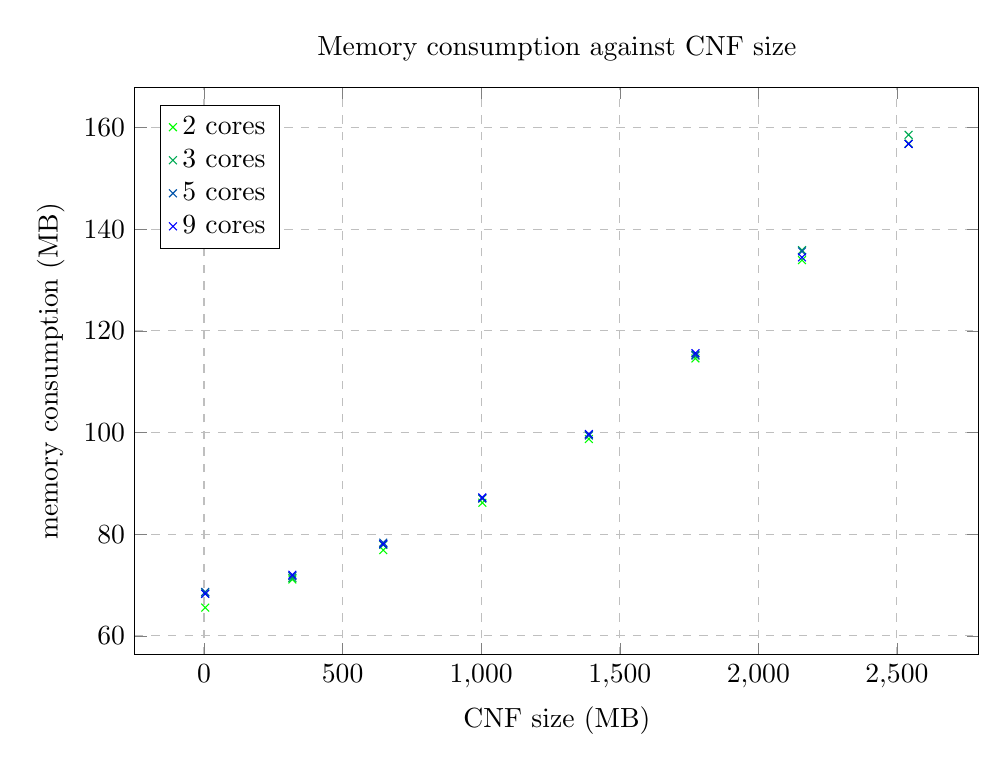
\begin{tikzpicture}
		\begin{axis}[
			title={Memory consumption against CNF size},
			xlabel={CNF size (MB)},
			ylabel={memory consumption (MB)},
			%xmin=0, xmax=0.25,
			%ymin=10.00, ymax=100000.00,
			%ymode=log,
			%xmode=log,
			%xtick={0,0.05,0.1,0.15,0.2,0.25},
			%ytick={0,20,40,60,80,100},
			%yticklabel=$\pgfmathprintnumber{\tick}\%$,
			legend pos=north west,
			ymajorgrids=true,
			xmajorgrids=true,
			grid style=dashed,
			xticklabel style={/pgf/number format/fixed},
			width = 350,
			height = 250
		]



\addplot[color=blue!0!green,only marks,mark=x] coordinates {
(4.1669921875,65.5703125)(318.771484375,71.09375)(646.669921875,76.87890625)(1004.0185546875,86.203125)(1388.5263671875,98.7421875)(1773.03515625,114.58984375)(2157.5439453125,133.93359375)(2542.052734375,156.85546875)
}node[pos=0.8](endofplotsquare){} ;
\addlegendentry{2 cores}
\addplot[color=blue!33!green,only marks,mark=x] coordinates {
(4.1669921875,68.35546875)(318.771484375,71.37109375)(646.669921875,77.9296875)(1004.0185546875,87.015625)(1388.5263671875,99.54296875)(1773.03515625,115.32421875)(2157.5439453125,135.91015625)(2542.052734375,158.578125)
}node[pos=0.8](endofplotsquare){} ;
\addlegendentry{3 cores}
\addplot[color=blue!67!green,only marks,mark=x] coordinates {
(4.1669921875,68.64453125)(318.771484375,71.76171875)(646.669921875,78.34765625)(1004.0185546875,87.07421875)(1388.5263671875,99.421875)(1773.03515625,115.16015625)(2157.5439453125,135.640625)(2542.052734375,156.77734375)
}node[pos=0.8](endofplotsquare){} ;
\addlegendentry{5 cores}
\addplot[color=blue!100!green,only marks,mark=x] coordinates {
(4.1669921875,68.26171875)(318.771484375,72.02734375)(646.669921875,78.0703125)(1004.0185546875,87.23828125)(1388.5263671875,99.71875)(1773.03515625,115.62109375)(2157.5439453125,134.48046875)(2542.052734375,156.8046875)
}node[pos=0.8](endofplotsquare){} ;
\addlegendentry{9 cores}





		\end{axis}
		\end{tikzpicture}
		%\vspace{-18pt}
  \caption{\dagster\ memory consumption for conjunctions of large-easy problems against core count.\label{fig:memory_consumption}}
    \end{figure}
